\section{System Design}
\label{cha:systemdesign}

Based on the requirements for FaaS platforms on the edge that we identified in \cref{cha:background}, we have developed \textit{tinyFaaS}, a FaaS platform that is built from the ground up for edge environments.

\begin{figure}
    \centering
    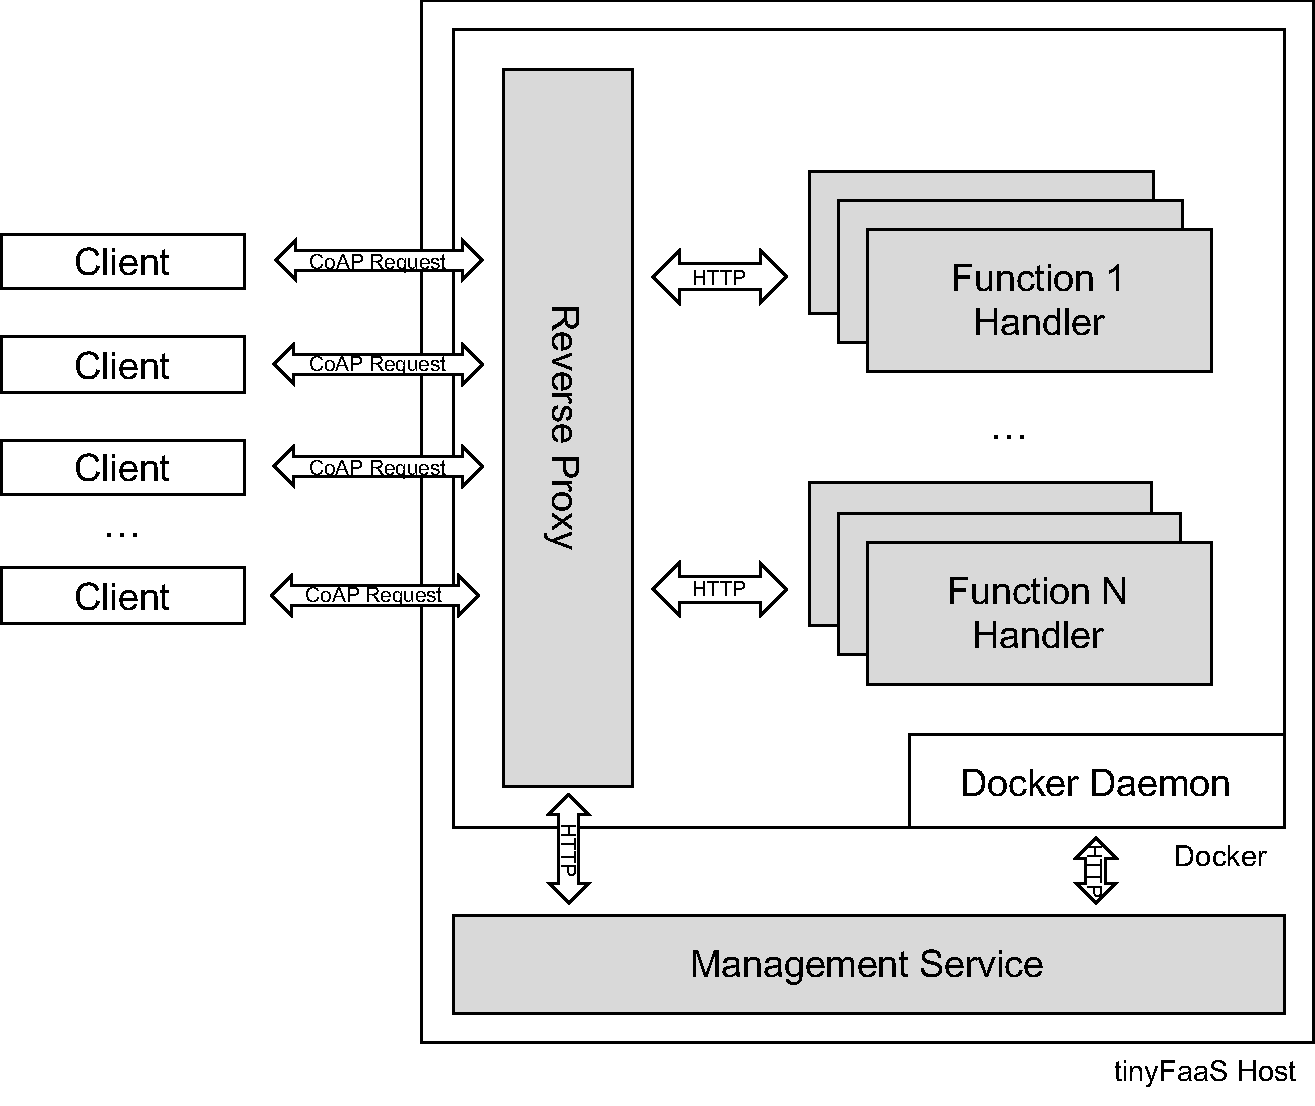
\includegraphics[width=0.66\columnwidth]{fig/architecture.pdf}
    \caption{\textit{tinyFaaS} Architecture}
    \label{fig:systemdesign}
\end{figure}

In this section we will present the architecture of \textit{tinyFaaS}, which is shown in \cref{fig:systemdesign}.
Its main components are a reverse proxy that acts as a CoAP proxy and load balancer, function handlers that execute the application code, and a management service to supervise the other components.

As each of these components communicates using standard web protocols, they are easily interchangeable as well, which further increases extensibility.
For example, the reverse proxy, which accepts incoming CoAP connections, could easily be replaced with an HTTP proxy for less latency-sensitive applications or to integrate it into legacy systems.
While \textit{tinyFaaS} is designed to run on a single node, it is also possible to integrate multiple nodes in a common middleware or through an external load balancer by extending the management service or reverse proxy.

\subsection{Reverse Proxy}
\label{sec:reverseproxy}

The reverse proxy accepts incoming CoAP connections and proxies them to the function handlers.
For each function, a CoAP resource is registered in the reverse proxy and requests to that resource are treated as a call to the corresponding function.
When a message reaches the CoAP endpoint, the reverse proxy selects one of the function handlers to process this request.
The reverse proxy then sends an HTTP request, possibly with some meta-information or data, to the HTTP proxy in the selected function handler.

As we have discussed in \cref{sec:focus_on_iot}, a FaaS platform for the edge should natively support messaging protocols that are used for machine-to-machine communication and fit the IoT use case as well.
We decided to use CoAP as the messaging protocol for \textit{tinyFaaS} for several reasons.
First, CoAP, which is short for \textit{Constrained Application Protocol} follows the client/server paradigm in the style of HTTP, compared to the publish/subscribe approach that MQTT takes.
This fits our use case as we expect clients such as IoT devices to send requests to the server that hosts \textit{tinyFaaS} without the need for a common message broker.
Second, CoAP is very efficient and lightweight.
All other factors being equal, it introduces much lower latency overheads and can sustain higher throughput levels compared to HTTP and MQTT.
These lower resource needs are mainly due to CoAP using UDP at the transport layer.
As TCP is connection-oriented, it introduces a lot of overhead; UDP, in contrast, does not use a controlled connection between the two communicating parties.
This not only greatly reduces how much processing is needed for each CoAP packet but also reduces network bandwidth usage~\cite{Laaroussi2018-fk,Naik2017-cn}.


\subsection{Function Handlers}
\label{sec:handlers}

\begin{figure}
    \centering
    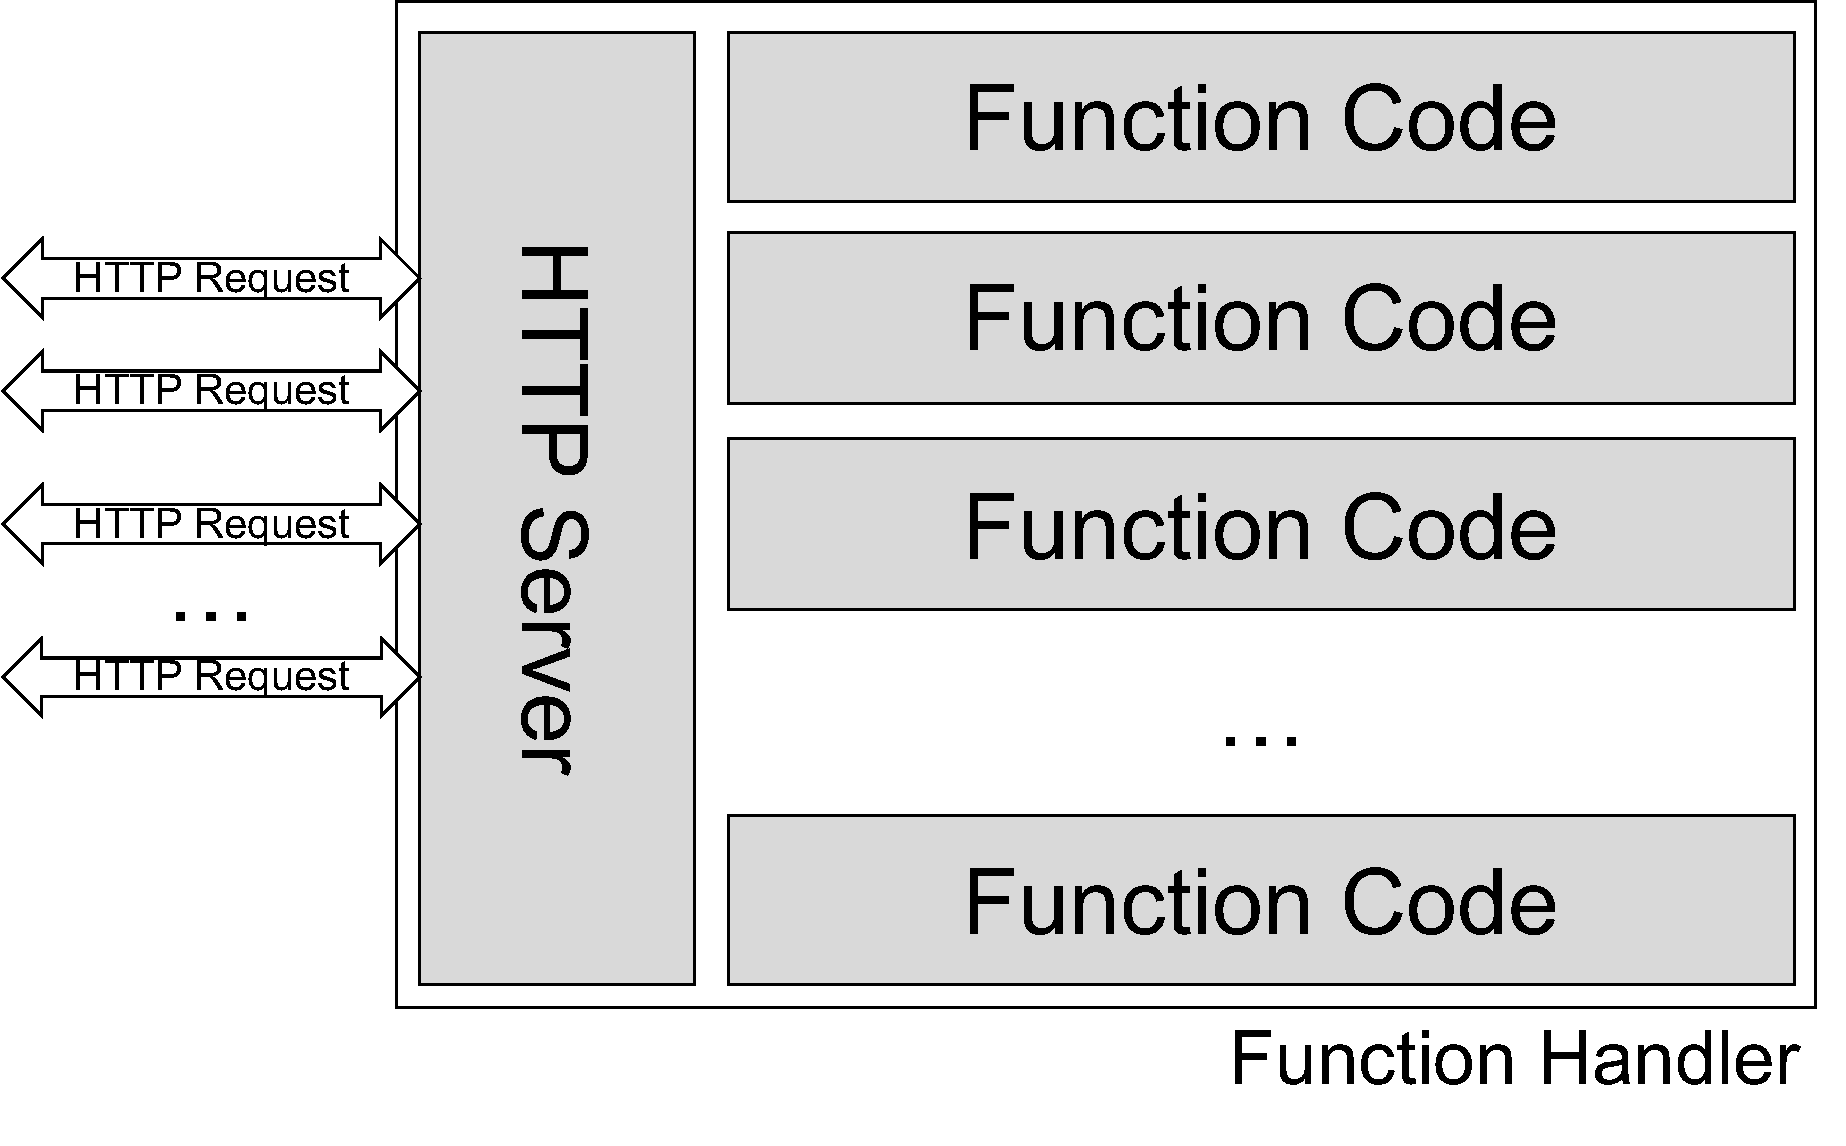
\includegraphics[width=0.66\columnwidth]{fig/functionhandler.pdf}
    \caption{Components of the Function Handler}
    \label{fig:functionhandlers}
\end{figure}

The function handlers are the main part of \textit{tinyFaaS}.
Each function handler is a separate Docker container.
This container contains both a runtime for the programming language that the function is written in and some boilerplate code to facilitate calling it from the reverse proxy.
As shown in \cref{fig:functionhandlers}, the container also includes an HTTP server that accepts incoming requests from the reverse proxy, executes the function with the data provided by the request and returns a result.
While the reverse proxy uses CoAP for external communication, HTTP is used internally within \textit{tinyFaaS}.
Using an HTTP server for communication between the reverse proxy and the function handlers makes it very simple to add new function runtimes, as most modern runtimes support some form of HTTP server out of the box with standard libraries, which is not necessarily the case for CoAP.
Using HTTP here, therefore, improves extensibility.
As the reverse proxy and function handlers run on the same physical host and are connected directly with a virtual network, the communication overhead is negligible.
Furthermore, the connection can be reused for every (internal) request.

Each function handler can accept an arbitrary number of concurrent incoming requests.
Consequently, requests within one container are isolated from each other only on an application level by using threads, yet not on an operating system level.
The trust boundary is set at a function level rather than at request level.
While creating a new Docker container for each request would increase isolation, it results in a considerably higher performance overhead and less efficient resource allocation.
We believe that this is ``good enough'' in terms of a trust model.

Consider the following example: A function developer D develops and deploys a function which is used by users U1 and U2.
In this scenario, neither U1 nor U2 can directly access each other's data without involving D.
D, however, needs to be trusted by both users anyhow as they could leak tenant data in other ways as well.
This only leaves the question of a buggy function that leaks information which, however, cannot be properly exploited by either user as such a bug would go in both directions.
Furthermore, in a stateless programming model, this is also very likely to materialize as a malfunction.

Overall, we believe that this suffices for our purposes; there may, however, be scenarios where more isolation at the cost of performance is needed -- these can simply be addressed by routing requests of the respective user (who is unlikely to attack himself) to a dedicated container.
Nevertheless, this means that applications that run on \textit{tinyFaaS} must be developed for safe memory access so as not to interfere with itself when called concurrently.
Across different functions and, by extension, tenants, \textit{tinyFaaS} asserts isolation using Docker containers.
Through isolated runtimes, different function handlers cannot access other function's memory or files and the virtual networks prevent direct calls between them.
This ensures that no maliciously acting function can interfere with other functions.

While Docker containers only introduce a small performance penalty, they dramatically simplify deployment of functions as the corresponding handlers and dedicated virtual networks can easily be created in an isolated fashion by the management service.

\subsection{Management Service}
\label{sec:management}

The management service is responsible for creating new functions within the platform.
Developers who want to deploy a new function can send it the management service' HTTP endpoint.
The service then creates the containers for the function handlers, registers a CoAP resource in the reverse proxy, and connects all handlers with the reverse proxy on a Docker virtual network so that they can communicate.
Similarly, functions may also be updated or deleted.
This allows functions on \textit{tinyFaaS} to be reconfigured at runtime, which is a key feature of FaaS platforms.

Furthermore, having a single point of entry also enables multi-tenancy as the management service can take care of user authentication when creating or modifying functions.
While it would be possible to integrate this into the reverse proxy, as we tried in an earlier prototype, having the management service as a separate component has two advantages.
First, it keeps the reverse proxy as slim as possible, making it more resource efficient.
Second, having separate components allows us to replace individual components.
For instance, it is possible to configure \textit{tinyFaaS} by sending HTTP requests to the host's Docker daemon and the existing \textit{tinyFaaS} reverse proxy.
This allows us to easily replace the management service, e.g., with an external or distributed service which would add remote management capabilities to our system.
